\documentclass[12pt, english]{report}
\usepackage{subcaption}
\usepackage{amsmath}
\usepackage{amssymb}
\usepackage{stackrel}
\usepackage{graphicx}
\usepackage{hyperref}
\usepackage{caption}
\usepackage[noadjust]{cite}
\usepackage{authblk}
\usepackage{placeins}
\usepackage{adjustbox}
\usepackage{tabularx}
\usepackage{graphics}
\usepackage[nottoc]{tocbibind}
\usepackage{ragged2e}
\usepackage{etoolbox}
\usepackage{subcaption}
\usepackage{float}
\usepackage{babel}
\usepackage[a4paper, total={6in, 10in}]{geometry}
\usepackage{booktabs}
\usepackage{colortbl}
\usepackage{xcolor}
\usepackage{xfrac}
\usepackage{listings}
\usepackage{color} %red, green, blue, yellow, cyan, magenta, black, white
\definecolor{mygreen}{RGB}{28,172,0} % color values Red, Green, Blue
\definecolor{mylilas}{RGB}{170,55,241}


\lstset{language=Matlab,%
    %basicstyle=\color{red},
    breaklines=true,%
    morekeywords={matlab2tikz},
    keywordstyle=\color{blue},%
    morekeywords=[2]{1}, keywordstyle=[2]{\color{black}},
    identifierstyle=\color{black},%
    stringstyle=\color{mylilas},
    commentstyle=\color{mygreen},%
    showstringspaces=false,%without this there will be a symbol in the places where there is a space
    numbers=left,%
    numberstyle={\tiny \color{black}},% size of the numbers
    numbersep=9pt, % this defines how far the numbers are from the text
    emph=[1]{for,end,break},emphstyle=[1]\color{red}, %some words to emphasise
    %emph=[2]{word1,word2}, emphstyle=[2]{style},
}



%%%%%%%%%%%%%%%%%%%%%%%%%%%%%%%%%%%%%%%%%%% for fonts of Abstract  %%%%%%%%%%%%%%%%%%%%%%%%%%%%%%%%%%%%%%%

\usepackage{abstract}
\renewcommand{\abstractnamefont}{\huge\bfseries}


%%%%%%%%%%%%%%%%%%%%%%%%%%%%%%%%%%%%%%%%%%%%%   Adding Biblography/lof/lit in table of content  %%%%%%%%%%%%%%%%%%%%%%%%%%%%%%%%%%%%%%%%%%%%%%%
%\usepackage{tocbibind}

\makeatletter

\begin{document}


\begin{titlepage}
\begin{center}



\includegraphics[width=0.35\textwidth]{./logo}~\\[1.5cm]

%%%%%%%%%%%%%%%%%%%%%%%%%%%%%%%%%%%%%%%%%%%%%%%%%%%%%%%%%%%%%%%%%%%% Title  %%%%%%%%%%%%%%%%%%%%%%%%%%%%%%%%%%%%%%%%%%%%%%%%%%%%%%%%%%%%%%%%%%%%

{ \huge \bfseries Electronic Voting Machine(EVM) Using 8051 Microcontroller} \\[1.4cm]

{ \large \bfseries Submitted by:} \\[0.2cm]
{ \large \bfseries Hamza Umar}  \\[0.1cm]
{ \small FA19-BCE-026} \\[0.2cm]
{ \large \bfseries Muhammad Kaleem Ullah}  \\[0.1cm]
{ \small FA19-BCE-007} \\[0.2cm]
%{ \small \bfseries Usman} \\[0.2cm]
%{ \small \bfseries Kashif} \\[0.2cm]



{ \small \bfseries Program: BS in Computer Engineering} \\[0.2cm]
%{ \small \bfseries Enrollment Number: 1234} \\[1.0cm]


{ \large \bfseries Submitted to:} \\[0.1cm]
{ \small \bfseries  Dr.Wasiq Ali} \\[0.1cm]
{ \small \bfseries Engr. Iram Shehzadi} \\[0.8cm]
%{ \large \bfseries Assistant Professor} \\[0.9cm]
%{ \large \bfseries Department of Electrical Engineering} \\[0.3cm]

\vfill

\textsc{A Project submitted in partial fulfillment of the requirements for the degree of bachelors of Science in Computer Engineering}\\[1cm]


{ \large \bfseries Department of Electrical and Computer Engineering} \\[0.2cm]
{ \large \bfseries COMSATS University Islamabad, Attock Campus, Pakistan.} \\[0.2cm]


% Bottom of the page
%{\large \today}   % Date

\thispagestyle{empty}
\end{center}
\end{titlepage}

% Thesis Dedication ---------------------------------------------------

%\begin{declaration} %this creates the heading for the dedication page
%\chapter*{Declaration}
%\begin{titlepage}

%\noindent {\Large \textbf{Declaration}} \\

%\vspace*{7cm}
\begin{titlepage}
\begin{center}
\noindent {\Large \textbf{Declaration}} \\
\end{center}
  \vspace*{0.5cm}

\noindent I declare that the project "Electronic Voting Machine (EVM) Using 8051 Microcontroller" is based on our own work carried out during the course of our study under the supervision of Dr. Wasiq Ali and Engr. Irum Shehzadi. \\
I assert the statements made and conclusions drawn are an
outcome of my research work. I further certify that\\[0.2cm]

\begin{enumerate}
\item  The work contained in the report is original and has been
done by us under the general supervision of my
supervisors.

\item The work has not been submitted to any other Institution
for any other degree/diploma/certificate in this university
or any other University of Pakistan or abroad.


\item We have followed the guidelines provided by the
university in writing the report.

\item Whenever we have used materials (data, theoretical
analysis, and text) from other sources, we have given due
credit to them in the text of the report and giving their
details in the references.

\end{enumerate}


\end{titlepage}
%\end{declaration}

% ----------------------------------------------------------------------

%\input{PrePages/CertificateofApproval}
%\input{PrePages/PlagiarismUnderTaking}
%\input{PrePages/ListOfPublications}
% Thesis Dedication ---------------------------------------------------

%\begin{dedication} %this creates the heading for the dedication page
%\chapter*{Dedication}
%\begin{titlepage}

%\noindent {\Large \textbf{Dedication}} \\

%\vspace*{7cm}
\begin{titlepage}
\begin{center}
\noindent {\Large \textbf{Dedication}} \\
\end{center}
  \vspace*{0.5cm}

\noindent First and foremost we offer our sincerest gratitude to our course instructor,  Dr.Wasiq Ali, and Lab instructor, Engr. Irum Shehzadi, Who encouragement, guidance and support from the initial to the final level enabled us to develop an understanding of the subject. Without his guidance and persistent help this project would not have been possible.\\\\
To our parents, we would like to thank to them for supporting us in our daily lives, for going to school every day, and having them by our side to guide us always, their prosperity and love for us.
\end{titlepage}
%\end{dedication}

% ----------------------------------------------------------------------

%%% Local Variables:
%%% mode: latex
%%% TeX-master: "../thesis"
%%% End:

\begin{titlepage}
\begin{center}
\noindent {\Large \textbf{Acknowledgements}} \\
\end{center}
  \vspace*{0.5cm}
\noindent Thanks to ALLAH (s.w.t), the Greatest, the most Merciful and the most Gracious, Whose countless blessings bestowed upon me kind, talented and wise teachers, who provided me sufficient opportunities, and enlighten me towards this research work.\vspace{.25cm}

\noindent I would like to extend my deepest thanks to our project supervisors, Dr.Wasiq Ali, and Engr. Irum Shehzadi for giving us the opportunity of undertaking this project under his determined directions. His support, dedication, encouragement, excellent supervision and guidance are what made this thesis possible. \vspace{.25cm}

\noindent Thanks to my beloved family, whose prayers, dedication, support and love are the most precious assets, I had (and I have), during the course of my Engineering work and for all of my endeavors.\vspace{.25cm}

\noindent I am very thankful to the administration and faculty of COMSATS University Islamabad, Attock Campus for providing me a great environment that helped me a lot in conducting our project related activities. \vspace{5mm} \\


\noindent Thank You!

%I am also extremely thankful to Dr. Waseem Ikram, Dr. Aftab Maroof, Dr. Arshad A. Shahid, Dr. Anwar M. Mirza, Dr. Farrukh A. Khan, Dr. Hammad Majeed and Dr. Waseem Shahzad for supporting me in my research work at NUCES.  How can I forget my colleagues (@ FAST): Muhammad Sharif, Mohsin Bilal, Asif Khan, Muhammad Ishtiaq, Hamid, Sajid, Javed, Ahmad, Hameed, Imran, Raees, Israrullah, Israr and all other PhD fellows for their support: intellectually as well as for the stuff, related to enjoyment!\vspace{.25cm}

%\noindent I am extremely thankful to my wife for helping me out in difficult situations. Also, thank you my sister for your love and for cooking the delicious foods that helped me in cooking the recipes of my ideas.\vspace{.25cm}

%\noindent And of course, even if I don't mention, they will get it: a big thank you to my friends: Javed Akhter, M. Nadeem Shahid, Arshad, Rana Khalil, Imran Niazi and M. Imran (hey, order doesn't matter) for offering outdoor enjoyment stuff that is difficult to be mentioned in this tiny document.\vspace{.25cm}

%\noindent Finally, I would like to gratefully acknowledge the financial support received from the Higher Education Commission of Pakistan during the course of my PhD (for almost everything).


\end{titlepage}


\begin{abstract}
\noindent We can experience fast and sudden changes in the life of human being due to the
information technology (IT). Information technology is used individually as well
as in business then how it could be exception for election. Information technology is useful in preparing voters list, proper voting and prediction of which candidate will be winner etc\cite{nikamcritical}.
EVM stands for Electronic voting Machine. This makes polling much fast and is more reliable than ballot papers, by preventing bogus voting to a great extend. The EVMs saves considerable time, money, and manpower. It also helps in maintaining the secrecy of individual voting. At the end of polling, just press a button and there you have the result.\\\\

\noindent Electronic Voting Machine(EVM) is a simple electronic device used to record votes in place of ballot papers and boxes which were used earlier in conventional voting system. Fundamental right to vote or simply voting in elections forms the basis of democracy. All earlier elections be it state elections or centre elections a voter used to cast his/her favorite candidate by putting the stamp against his/her name and then folding the ballot paper as per a prescribed method before putting it in the Ballot Box. This is a long, time-consuming process and very much prone to errors. This situation continued till election scene was completely changed by electronic voting machine. No more ballot paper, ballot boxes, stamping, etc. \\\\

\noindent All this condensed into a simple box called ballot unit of the electronic voting machine. Because biometric identifiers cannot be easily misplaced, forged, or shared, they are considered more reliable for person recognition than traditional token or knowledge based methods. So the Electronic voting system has to be improved based on the current technologies viz., biometric system \cite{kumar2012electronic}.\\\\
\noindent Due to EVM following points become possible:\\ 
\begin{itemize}
\item Fast counting of voting
%
\item Accurate counting of voting
%
\item Avoidance of misbehavior/misconduct
%
%
\end{itemize}

\vspace{0.89mm}
%\pagenumbering{roman}% added the roman page number in the starting pages
\thispagestyle{empty}% to remove the page number
\end{abstract}

%\input{PrePages/emptypage}
%\input{PrePages/Examiners}
%\input{PrePages/Certificate}

\pagenumbering{roman}
\setcounter{page}{11}


\tableofcontents{}
\pagebreak{}
%\listoffigures{}
\pagebreak{}
%\listoftables{}
\pagebreak{}
%\input{PrePages/nomenclature}
%\newpage{}
%\input{PrePages/ListofAbbreviations}


\pagenumbering{roman}
\setcounter{page}{23}

\newpage{}
\pagenumbering{arabic}

%%%%%%%%%%%%%%%%%%%%%%%%%%%%%%%%%%%%%  Chapters  %%%%%%%%%%%%%%%%%%%%%%%%%%%%%%%%%%%%%%%%%%%%%%%%%%%%%%%%%%%%%%%%%

\chapter{Introduction}
\label{chap1}
It is very critical and important to cast and count votes, the electronic voting is a term used to describe the act of voting
using electronic systems. Electronic Voting Machine (EVM) is an electronic device used
for recording votes. An Electronic Voting Machine consists of
two Units first is Control Unit and second is Balloting Unit that are joined by a 5 meter cable. The candidate names and symbol are programmed in the control unit of EVM. The polling officer in-charge of the control unit will release a ballot instead of issuing a ballot paper by pressing the ballot button on the control unit. This mechanism will enable the voter to cast his vote by pressing the blue button on the balloting unit against the candidate and symbol of his choice. \cite{nikamcritical}
\begin{figure}[H]  %h=positioning
\begin{center}
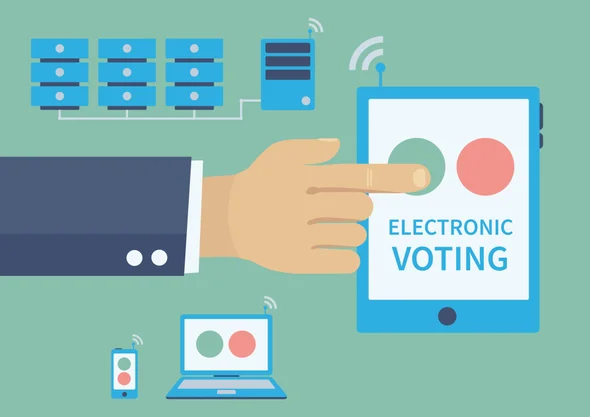
\includegraphics[scale=1.0]{Chapter1/evm}
\caption{Electronic Voting Machine (EVM)}
\label{figure1}
\end{center}
\end{figure}

\section{Objectives}
%
%
The objectives of this project are:
%
%for 1,2,3 numbers
\begin{enumerate}
\item To make elections time efficient and  cost efficient.
%
\item To eliminate the chance of rigging in the elections.
%
\item To automate the elections.
%
%
\end{enumerate}
\section{Introduction}
\noindent Elections allow the people to choose their representatives and express their preferences for how they will be governed. Naturally, the integrity of the election process is fundamental to the integrity of democracy itself. The election system must be sufficiently robust to withstand a variety of fraudulent behaviors and must be sufficiently transparent and comprehensible that voters and candidates can accept the results of an election.
Electronic voting refers to the use of computers or computerized voting equipment to cast ballots in an election. Sometimes, this term is used more specifically to refer to voting that takes place over the Internet\cite{kumar2012electronic}.

The design of a �good� voting system, whether electronic or using traditional paper ballots or mechanical devices, must satisfy a number of sometimes competing criteria.
\begin{itemize}
\item The anonymity of a voter�s ballot must be preserved
%
\item both to guarantee the voter�s safety when voting against a malevolent candidate
%
\item guarantee that voters have no evidence that proves which candidates received their votes
%
%
\end{itemize}
\begin{figure}[H]  %h=positioning
\begin{center}

\includegraphics[scale=2]{Chapter1/pic1}
\caption{EVM}
\label{figure1}
\end{center}
\end{figure}
The voting system must also be tamper-resistant to thwart a wide range of attacks, including ballot stuffing by voters and incorrect tallying by insiders. Another factor, as shown by the so-called �butterfly ballots� in the Florida 2000 presidential election, is the importance of human factors. A voting system must be comprehensible to and usable by the entire voting population, regardless of age, infirmity, or disability. Providing accessibility to such a diverse population is an important engineering problem and one where, if other security is done well, electronic voting could be a great improvement over current paper systems. Flaws in any of these aspects of a voting system, however, can lead to indecisive or incorrect election results.\cite{kohno2004analysis}


\section{E-Voting Systems}
It is also known as e-voting is a term encompassing several different types of voting, embracing both electronic means of casting a vote and electronic means of counting votes. Electronic voting technology can include punched cards, optical scan voting systems and specialized voting kiosks (including self-contained direct-recording electronic voting systems, or DRE). It can also involve transmission of ballots and votes via telephones, private computer networks, or the Internet. And, of course, EVM helps maintain total voting secrecy without the use of ballot papers. And, at the end of the polling, just press a button and
there you have the results.\cite{kumar2012electronic}


\section{Challenges}
\noindent The challenges are even harder because there is little or no training available for voters. The first time most voters ever touch the voting system is the moment they vote. And once they start voting, there is tremendous social pressure to do it without help. With people watching, inadequately trained poll workers, busy people waiting on line, the social importance of voting, and the value placed on secrecy, voters may become anxious and afraid to ask for help. Finally, the systemic issues of how voting machines get purchased and evaluated are problematic as well. State or county purchasers are usually more concerned about cost than usability. And once the systems are purchased, the public has no access to the machines for evaluation. Election workers who design ballots tend not to have experience in usability and screen design. Poll workers who deploy the voting systems have minimal training to cope with the inevitable problems. Electronic voting systems offer promise as well � from the opportunity to change font size and language on demand, to offering disabled users customized access, to accurate and fast recording and tabulation of votes. But there are many issues that add up to the risk that voters may become disenfranchised. And this is especially true for the elderly
and citizens at the margins of society.\cite{bederson2003electronic}

\subsection{Accountability and Verifiability}
Traditionally, votes were cast on paper and counted by hand. Voters were confident that the marks they made on ballots reflected their intended vote. Voting machines that used levers and punch card systems also provided voters with a high degree of confidence that they cast their votes as intended. In 2000, the U.S. presidential election was particularly contentious because the outcome was extremely close. This resulted in a close examination of the voting and tabulation systems that were used. Many problems were found, especially with one ballot design which became known as the �butterfly� ballot. This ballot required voters to draw line connecting a candidate with a circle. This was confusing because the circles didn't align well with the candidates and in addition, the circles were shared between two columns of candidates. The ensuing melee brought a popular awareness of the complexities and flaws in voting systems and there were general calls for reform. Many questions have since been raised.
Because they are paperless, systems raise the question:
 %for 1,2,3 numbers
\begin{enumerate}
\item How can one know that when a voter chooses a particular candidate on the screen?
%
\item Is a vote for that candidate is recorded?
%
\end{enumerate}
A simple solution to this problem is to provide the user with a printed record of the votes electronically recorded. Before leaving the polling place, the voter would be required to certify the contents of the paper record and place it into a ballot box. The printed records could then be manually counted in the event of a challenge, and this procedure would foil any attempt at falsifying votes
internally to the voting system. This approach, however, has not been implemented in any commercial systems that we are aware of\cite{bederson2003electronic}.

%\section{Motivation}
%Motivated by the emergence of technological advancements and challenges in ...


%
%

%
%\section{UN Stainability Goals}

 %Goal 8 is shown which is Promote sustained, inclusive and sustainable economic growth, full and productive employment and decent work for all. As we will also discuss the economical long time benefits in next chapters. Our project will help industry in economic growth as well as it is providing a help to the meter readers.



%The conceptual frame work for the proposed method is comprises of three basic building blocks and detailed model is shown in Fig. \ref{fw}.
%\begin{enumerate}
%\item Network Formation Block.
%\item Neighbourhood Based Network Matrix Formation Block.
%\item Consensus Formation Block.
%\end{enumerate}
%
%In the network formation block, ...
%
%\FloatBarrier
%\begin{figure}[H]
%\begin{center}
%\hspace{15mm}
%\includegraphics[scale=0.35]{Chapter1/robocanesinternalstates}
%
%\protect\caption{Pseudo-code of Proposed Scheme for Cooperative Control of Networked Multi-Agent Systems.}
%\label{scode}
%\end{center}
%\end{figure}
%
%
\section{Report Break Down}
%
%This thesis deals with convergence analysis .... The main contributions of this work are summarized as follows:
%
%\begin{enumerate}
%\item  Initially a design ....
%
%\item An extended ....
%
%
%\item Modeled a ....
%
%\end{enumerate}
%
%The main contribution of this work is to propose a new way ....
%
%
%
%
%\section{Thesis Outline}
%
%
The major focus of this report is on the findings of the proposed project i.e. Electronic Voting Machine(EVM) Using 8051 Microcontroller.\\

\noindent This Report is organized as follows:
\vspace{5mm}

\noindent In chapter 2, literature review is provided in detail about the work which is already been done on Electronic Voting Machine(EVM) Using 8051 Microcontroller and will give a brief details about the articles, papers and literature review.
\vspace{5mm}


\noindent In Chapter 3, Proposed Methodology is presented in which you will be able to see the method we will work on the designing of a complete project source code to the diagrams.

\vspace{5mm}


\noindent In Chapter 4, Result and Simulations are being discussed, in which you will see all kind of finding related to the Electronic Voting Machine(EVM) Using 8051 Microcontroller.


\vspace{5mm}

\noindent In Chapter 5, we have concluded and summarized the project work and also presented few new research ideas for future studies.


%\begin{equation}
%F=\sum_{n=0}^i(x_i(0)-x_j(0))^2
%%stackrel[u]{v}{T}=\stackrel[u]{v}{L}+\stackrel[u]{v}{L}\underset{W\epsilon V\cap w\neq u}{\sum}\stackrel[v]{w}{L}
%\end{equation}

\chapter{Literature Review}
\label{chap2}

In the chapter 1 we have given the introduction of our project, objectives and a thesis break down. Our introduction chapter is giving a complete overview of this project report. This chapter is about the work which is already been done on Electronic Voting Machine and will give a brief details about the articles, papers and literature review.

\section{Literature Review}
Researchers in the electronic voting field have already reached a consensus pack of following core properties that an electronic voting system
should have\cite{kumar2012electronic}:
\subsection{Accuracy}
\begin{enumerate}
\item It is not possible for a vote to be altered.
%
\item It is not possible for a validated vote to be eliminated from the final tally.
%
\item It is not possible for an invalid vote to be counted in the final tally.
%
%
\end{enumerate}
\subsection{Democracy}
\begin{enumerate}
\item It permits only eligible voters to vote.
%
\item It ensures that eligible voters vote only once.
%
\end{enumerate}
\subsection{Privacy}
\begin{enumerate}
\item Neither authorities nor anyone else can link any ballot to the voter who cast it.
%
\item No voter can prove that he voted in a particular way.
%
\end{enumerate}
\subsection{Verifiability}
\begin{enumerate}
\item Anyone can independently verify that all votes have been counted correctly.

\end{enumerate}
\subsection{Availability}
\begin{enumerate}
\item The system works properly as long as the poll stands

\item Any voter can have access to it from the beginning to the end of the poll.

\end{enumerate}
\subsection{Resume Ability}
\begin{enumerate}
\item The system works properly as long as the poll stands

\item the system allows any voter who had interrupted his/her voting process to resume it or restart it
while the poll stands.

\end{enumerate}
\section{Features}
Following are some of the features which an electronic voting machine should have.
\begin{itemize}
\item There are no external communication paths hence it is difficult for the hackers to hack the machine and tamper the count numbers, in most of the advanced version of electronic voting machines.
%
\item Electronic voting machines with touch base screen are proven to be advantageous for the physically challenged people. In a paper ballot, these physically challenged people were not able to cast their votes in private. However, with the new EVM in place, even handicapped people can use their right to vote in private.
%
\item Electronic voting machines are cost effective and economical. In the paper ballot, the amount of raw material used is higher. It directly impacts the environment as paper ballot uses papers to cast votes. However, the cost associated with holding elections with EVMs is considered to be negligible.
%
\item One of the advantages of the electronic voting machine
is to save the time. EVM machines can cast and count the votes within very less time.
%
\item Bogus voting can be avoided through electronic voting machines hence are quite effective against the bogus votes. Electronic voting machines are programmed to capture a maximum of five votes in a minute, due to which a single vote cannot cast fake votes. In advanced electronic voting machines, a sound of beep comes after one casts their vote which lets the officer on duty know that the vote has been cast by an individual.
Electronic voting machines are designed in a way that they keep a track of number and details of votes recorded. The election commission can even save the data for a longer period of time which might be helpful for referencing in future.
%
\item Electronic voting machines are easier to carry and transport from one place to another without any hassle. One single machine can record several votes captured through that machine. Few electronic voting machines also come with a voice support to assist the visually impaired voter. In such cases, the visually challenged person can cast their vote without any problem.
\item One can see all the symbols and names in electronic voting machines of the candidates together which makes it easier for the voter to choose among the many and cast their votes.
%
\end{itemize}
\section{Limitations}
Following are the problems, error, and challenges of implementing Electronic Voting Machine(EVM)\cite{nikamcritical}.
\begin{enumerate}
\item With recent elections in the United States, many software programmers have claimed that the electronic voting machines are vulnerable to malicious programming and if it gets affected then any hacker can hack the machine and can tamper the vote counts easily.
%
\item The touch base screen is not efficient enough to capture the vote accurately for many physically challenged people as they have complained that. Therefore sometimes it leads to the voter ending up voting for someone else unintentionally.
%
\item Although it takes the time to count votes that were captured using paper ballot but people fully trust the process as high technology are also vulnerable to hackers attack.
%
\item The electronic voting machines which were used during the elections are susceptible to damage which will result in loss of data. Therefore biggest change with technology is that no matter how much data it records but a single virus can destroy the entire data storage.
%
\item The highly humid area and those areas which receive frequent rainfall are not suitable for casting votes using electronic voting machines. As machines are prone to damage due to high humidity level thus usage of electronic voting machines are not advisable in such areas.
%
\item Most of the electronic voting machines used in the country were foreign manufactured, which means the secret codes that control the electronic voting machines are in foreign hands and they can be used to influence the election results.
%
\item Fake display units could be installed in the electronic voting machines which would show manipulated
numbers but originally fake votes could be generated from the back end. This process does not need any hacker
to hack the software. Such fake display units are easily available in the market.
%
\item Most of the electronic voting machines used in the country do not have any mechanism by which the voter can verify their identity before casting the vote due to which fake voters can cast numerous fake votes.

\end{enumerate}

\noindent It is concluded that voting through electronic voting machine is need of time as all developed countries are making use of it. Researchers have been suggested an algorithm and are of opined that if suggested algorithm is strictly followed then there will not be any error in electronic voting procedure, and we will tackle all the mentioned above problems/issues\cite{nikamcritical}.






%\begin{table}[H]
%%\large
%\centering
%\caption{Consolidated Comparison of all the Systems}
%\label{tab2}
%%begin{adjustwidth}{-2.25in}{Oin}
%
%\begin{tabular}{|c|c|c|c|c|c|}
%\hline  %make a line
%Technology Used&Cost&Feasibility&Reliability&Communication Protocol\\
%\hline %make a line
%GSM&Low&Most Feasible&High&Stable\\
%\hline
%ZigBee&Medium&Small Scale&Low&Least Stable\\
%\hline
%SCADA&High&Not Feasible&High&Stable\\
%\hline
%PLC&Low&Least Feasible&Low&Very Stable\\
%\hline
%WiMAX&Medium&Small Scale&Medium&Stable\\
%\hline
%Mixed&Varies&Feasible&Varies&Varies\\
%\hline
%\end{tabular}
%\end{table}
%
%\small
%\begin{table}[H]
%\caption{Literature Review}
%\label{tab3}
%\centering
%\begin{tabularx}{1\linewidth}{X X X X}
%\toprule
% Paper Reference & Approach & Technology & Accuracy ($\%$) \\
%\toprule
%\cite{khan2020cost}&Cost Benefit Based Analytical Study of AMR and Blind Meter Reading (BMR) used by PESCO(WAPDA)& AMR and BMR &The Blind Meter Reading has internal financial return of about 84 percent while in case of AMR it is 15 percent.\\
%%\toprule
%\hline  %make a line
%\cite{zhao2005research} & Remote Meter Automatic Reading
%Based on Computer Vision & Computer vision techniques & $78\%$\\
%\hline %make a line
%\cite{li2019light} & Light-Weight Spliced Convolution Network-Based
%Automatic Water Meter Reading in Smart City & Network-Based
%Automatic Water Meter Reading & $85.66\%$ \\
%%\toprule
%\hline  %make a line
%\cite{dong2010design} & Wireless AMR System Based on SOPC & SOPC & $59.6\%$ \\
%\hline  %make a line
%\cite{ando2002automatic} & AMR system adopting automatic routing technology & routing technology & $68\%$ \\
%\hline  %make a line
%\cite{wiratama2018gas} & Gas
%billing system based on AMR on diaphragm gas meter with email
%notification & GSM or
%GPRS networks & $79\%$\\
%\hline  %make a line
%\cite{ashna2013gsm} & GSM based automatic AMR system with instant billing & GSM & $88\%$\\
%\hline  %make a line
%\cite{shuo2019digital} & Digital recognition of electric meter with deep learning & Deep Learning Methods & $78\%$\\
%\hline  %make a line
%\end{tabularx}
%\end{table}
%\small
%\begin{table}[H]
%\caption{-- continued from previous Literature Review table \ref{tab3}}
%\label{tab4}
%\centering
%\begin{tabularx}{1\linewidth}{X X X X}
%\toprule
% Paper Reference & Approach & Technology & Accuracy ($\%$) \\
%\toprule
%
%\cite{kulkarni2012gsm} &GSM based AMR system using ARM controller & ARM Controller & $81\%$\\
%\hline  %make a line
%\cite{Ali2012} & Implementation of (AMR) using radio frequency (RF) module & Radio Frequency & $58\%$\\
%\hline  %make a line
%\cite{palaniappan2015automated} & Comparison between different technologies being used in ARM  & GSM, Zigbee, SCADA System, Power Line Communication, WiMAX Technology,  & GSM = $88\%$, Zigbee = $67\%$,SCADA = $63\%$,Power Line = $71\%$,WiMAX = $62\%$,  \\
%\hline %make a line
%\cite{quan2010design} & Design of remote automatic meter reading system based on ZigBee and GPRS & ZigBee and GPRS techniques & $67\%$\\
%\hline  %make a line
%\cite{arun2012design} & Design and implementation of AMR system using GSM, ZIGBEE through GPRS & using GSM, ZIGBEE through GPRS & $89\%$\\
%\hline  %make a line
%\cite{rouf2012neighborhood} & Security and privacy analysis of automatic meter reading systems & Analysises of AMR & -\\
%\hline  %make a line
%\cite{malhotra2013automatic} & AMR and theft control system by using GSM & GSM & $84\%$\\
%\hline  %make a line
%\cite{tan2007automatic} & Automatic power meter reading system using GSM network & GSM network  & $78\%$\\
%\hline  %make a line
%\cite{Jamil2008} & Design and implementation of a wireless AMR system & GSM Network & $86\%$\\
%\hline  %make a line
%\cite{yuan2011remote} & Remote wireless AMR system based on GPRS & GPRS & $88\%$\\
%\hline  %make a line
%\cite{borle2013automatic} & AMR for electricity using power line communication & power line communication & $65\%$\\
%\hline  %make a line
%\end{tabularx}
%\end{table}
%\small
%\begin{table}[H]
%\caption{-- continued from previous Literature Review table \ref{tab4}}
%\label{tab5}
%\centering
%\begin{tabularx}{1\linewidth}{X X X X}
%\toprule
% Paper Reference & Approach & Technology & Accuracy ($\%$) \\
%\toprule
%\cite{mlakic2017designing} & Designing AMR system using open source hardware and software &open source hardware and software & $59\%$\\
%\hline  %make a line
%\cite{khalifa2010survey} & A survey of communication protocols for auto-
%matic meter reading applications, & Communication Protocols & - \\
%\hline
%\bottomrule
%\end{tabularx}
%\end{table}

%\section{Concluding Remarks}
%In this chapter, we have given a overall review about the literature related to Speech Processing Using MATLAB. MATLAB is a programming and numeric computing platform used by millions of engineers and scientists to analyze data, develop algorithms, and create models.\\\\
%In the chapter 3 we will proposed methodology which we will use for our project with block diagrams, flowcharts, Mathematical Modeling, escudo code and component selection related to the hardware and software.


\chapter{Proposed Methodology}
\label{chap3}
In the previous chapter, we have discussed the theories that support this research related to the Electronic Voting Machine . In this chapter we will proposed our methodology for this project.
\section{Block Diagram}
Let us look at the simplified block diagram in Figure \ref{blockDiagram}, which illustrates the main components involved
in Electronic Voting Machine(EVM) Using 8051 Micro-controller. Switches are used to make choices, resister, capacitor, and oscillator are being used to work the micro-controller properly on the circuits with the help of connecting wires.
\begin{figure}[H]  %h=positioning
\begin{center}
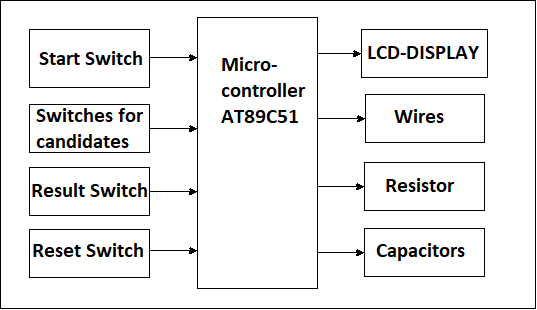
\includegraphics[scale=0.80]{Chapter3/blockDiagram}
\caption{Simplified Block Diagram of Electronic Voting Machine(EVM) Using 8051 Microcontroller}
\label{blockDiagram}
\end{center}
\end{figure}
\section{About Microcontroller 8051}
\noindent The 8051 Microcontroller was designed in the 1980s by Intel. Its foundation was on Harvard Architecture and was developed principally for bringing into play Embedded Systems. At first, it was created using NMOS technology but as NMOS technology needs more power to function therefore Intel re-intended Microcontroller 8051 employing CMOS technology and a new edition came into existence with a letter �C� in the title name, for illustration: 80C51. These most modern Microcontrollers need a fewer amount of power to function in comparison to their forerunners. There are many applications with an 8051 microcontroller.\\\\



\noindent The AT89C51 is a CMOS 8-bit microcomputer with 4K bytes of Flash programmable and erasable read only memory (PEROM).  The on-chip Flash allows the program memory to be reprogrammed in-system or by a ordinary nonvolatile memory programmer. Atmel AT89C51 is a powerful microcomputer/microcontroller (as they are used inter-changeably) which provides a highly-flexible and cost-effective solution to many embedded control applications.
\subsection{Features of AT89C51}
Following are some of the main feature of the used microcontroller i.e, AT89C51:
\begin{enumerate}
\item 8-bit CPU through two Registers A and B.
\item 8K Bytes � Internal ROM and it is a flash memory that supports while programming the system.
\item 256 Bytes � Internal RAM where the first RAM with 128 Bytes from 00H to 7FH is once more separated into four banks through 8 registers in every bank, addressable registers -16 bit \& general-purpose registers � 80.
\item The remaining 128 bytes of the RAM from 80H to FFH include Special Function Registers (SFRs). 
\item These registers control various peripherals such as Serial Port, Timers, all I/O Ports, etc.
\item Interrupts like External-2 \& Internal-3
\item Oscillator \& CLK Circuit.
\item Control Registers like PCON, SCON, TMOD, TCON, IE, and IP.
\item 16-bit Timers or Counters -2 like T0 \& T1.
\item Program Counter � 16 bit \& DPRT (Data Pointer).
\item I/O Pins � 32 which are arranged like four ports such as P0, P1, P2 \& P3.
\item Stack Pointer (SP) � 8bit \& PSW (Processor Status Word).
\item Serial Data Tx \& Rx for Full-Duplex Operation
\item a five vector two-level interrupt architecture
\item a full duplex serial port, on-chip oscillator and clock circuitry
%
\end{enumerate}
\section{Detailed Block Diagram - 8051}
Following is the detailed block diagram of the 8051.
\begin{figure}[H]  %h=positioning
\begin{center}
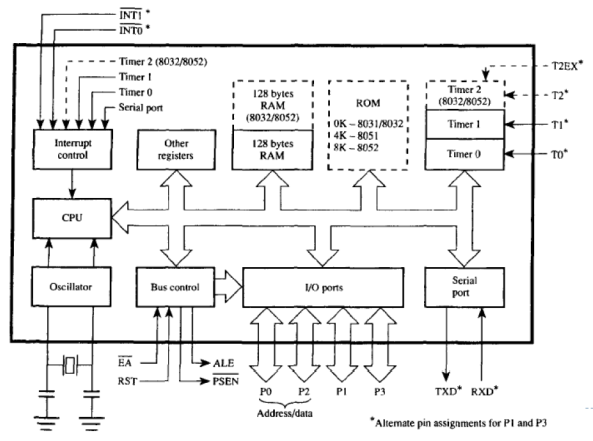
\includegraphics[scale=0.80]{Chapter3/blockDiagram8051}
\caption{Detailed Block Diagram of 8051 Microcontroller}
\label{blockDiagram8051}
\end{center}
\end{figure}
\subsection{Central Processor Unit (CPU)}
\noindent CPU is the brain of any processing device. It monitors and controls all operations that are performed in the Microcontroller. User has no control over the work of CPU. It reads program written in ROM memory and executes them and do the expected task.
\subsection{Interrupts}
\noindent Interrupt is a subroutine call that interrupts Microcontroller's main operation or work and causes it to execute some another program which is more important at that time. The feature of Interrupt is very useful as it helps in cases of emergency. Interrupts gives us a mechanism to put on hold the ongoing operation , execute a subroutine and then again resumes normal program execution The Microcontroller 8951 can be configured in such a way that it temporarily terminates or pause the main program at the occurrence of interrupt. When subroutine is completed then the execution of main program starts as usual. There are five interrupt sources in 8951 Microcontroller. 2 of them are external interrupts, 2 timer interrupts and one serial port interrupt.
\subsection{Input/output Port}
\noindent Microcontroller is used in embedded systems to control the operation of machines. Therefore to connect it to other machines, devices or peripherals we require I/O interfacing ports in Microcontroller. For this purpose Microcontroller 8951 has 4 input output ports to connect it to other peripherals.
Timers/Counters: Microcontroller 8951 has 2 16 bit timers and counters. The counters are divided into 8 bit registers. The timers are used for measurement of intervals, to determine pulse width etc.
\subsection{Oscillator}
\noindent Microcontroller is a digital circuit device, therefore it requires clock for its operation. For this purpose, Microcontroller 8951 has an on-chip oscillator which works as a clock source for Central Processing Unit. As the output pulses of oscillator are stable therefore it enables synchronized work of all parts of 8951 Microcontroller.
\subsection{Bus}
\noindent Basically Bus is a collection of wires which work as a communication channel or medium for transfer of Data. These buses consist of 8, 16 or more wires. Thus these can carry 8 bits, 16 bits simultaneously. Buses are of two types:
\begin{itemize}
\item Address Bus
%
\item Data Bus
%
\end{itemize}
\subsubsection{Address Bus}
Microcontroller 8051 has a 16 bit address bus. It used to address memory locations. It is used to transfer the address from CPU to Memory.
\subsubsection{Data Bus}
Microcontroller 8051 has 8 bits data bus. It is used to carry data.

\section{Pin Description 8051}
Following is the pin description diagram of the 8051
\begin{figure}[H]  %h=positioning
\begin{center}
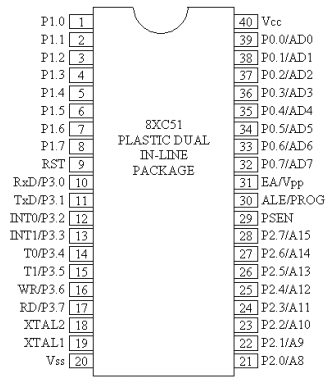
\includegraphics[scale=1.2]{Chapter3/pinDiagram}
\caption{Pin Diagram of 8051 Microcontroller}
\label{pinDiagram}
\end{center}
\end{figure}
\begin{figure}[H]  %h=positioning
\begin{center}
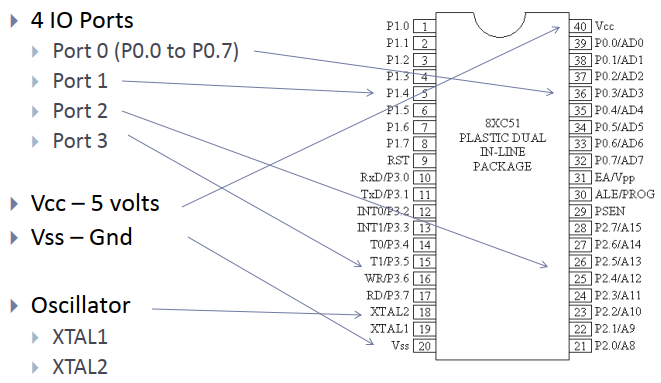
\includegraphics[scale=0.99]{Chapter3/pin1}
%\caption{Pin Diagram of 8051 Microcontroller}
%\label{pinDiagram}
\end{center}
\end{figure}
\begin{figure}[H]  %h=positioning
\begin{center}
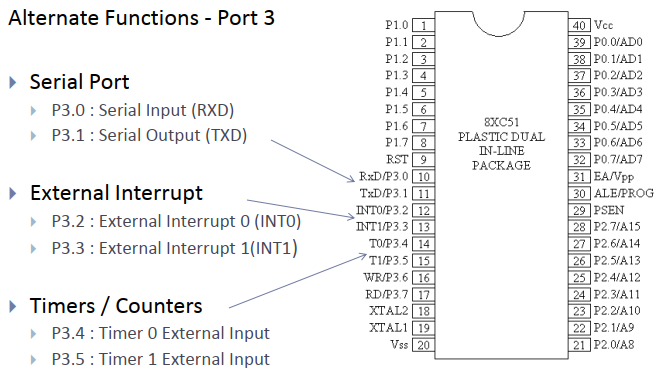
\includegraphics[scale=1.0]{Chapter3/pin2}
%\caption{Pin Diagram of 8051 Microcontroller}
%\label{pinDiagram}
\end{center}
\end{figure}
\begin{figure}[H]  %h=positioning
\begin{center}
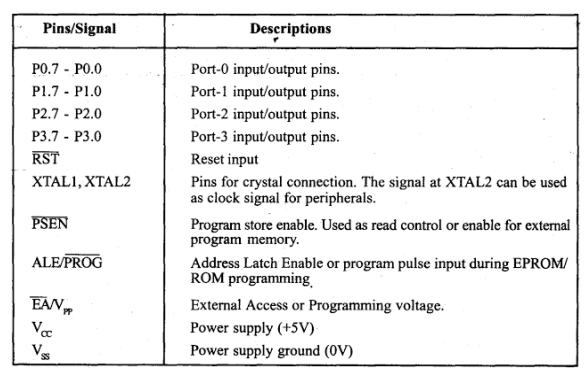
\includegraphics[scale=0.95]{Chapter3/pinsDetails}
\caption{Signals of 8031/8051 microcontroller of 8051 Microcontroller}
\label{pinsDetails}
\end{center}
\end{figure}
\begin{figure}[H]  %h=positioning
\begin{center}
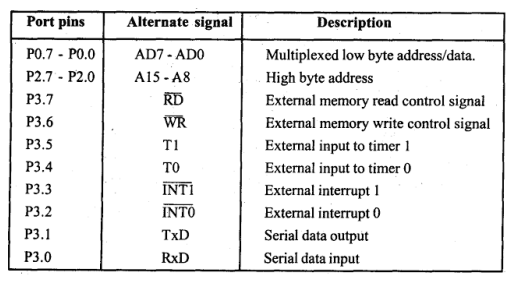
\includegraphics[scale=1.2]{Chapter3/pinsDetails1}
\caption{Alternate functions of port pins of 8051 Microcontroller}
\label{pinsDetails1}
\end{center}
\end{figure}

\subsection{Ports: (pin 1 to 8, pin 10 to 17, pin 21 to 28 and pin 32 to 39)}
\begin{itemize}
\item The 8031/8051 microcontroller has 32 I/O pins and they are organized as four numbers of 8-bit parallel
port.
\item The ports are denoted as port-0, port-1, port-2 and port-3. Each port can be used as either 8-bit parallel
port or 8 numbers of 1-bit ports.
\item The ports behave as latches during output operation and behave as buffers during input operation.
\item Port-1 can be used only for I/O operation
\item When external memory is employed, the port-0 function as multiplexed low byte address or data lines,
and port-2 function as high byte address lines. Therefore for accessing external memory the microcontroller
uses 16-bit address and access the memory in bytes. Hence the addressable memory space is 64 kb (216 =
64kb).
\item The 8031/8051 allows the external memory to be organized as two banks of 64 kb. One is program/code
memory and the other is data memory.
\end{itemize}
\subsection{PSEN (low signal): pin 29}
\begin{itemize}
\item The signal PSEN (low) is used as read control/enable for program memory.
RD (low signal) and WR (low signal): pin 17 and pin 16
\item The port pin P3.7 function as read control and the port pin P3.6 function as write control for data
memory.
\item When two external memory banks are not desirable, the PSEN (low) and RD (low) should be externally
ANDed to provide a single read control signal. In such cases the controller will access a common memory
space (of maximum capacity 64 kb) for program and data.
\item ALE is used to demultiplex the low byte address or data using an external latch.
\end{itemize}
\subsection{EA (Low)/Vpp : pin 31}
\begin{itemize}
\item When the microcontroller access program from external memory, then this pin is low. ie. EA (low) is
enabled.
\item When the microcontroller access program from internal memory, then this pin is high. At that time this
pin is used to supply programming voltage +12V to EPROM/ROM.
\end{itemize}
\subsection{XTAL 1 AND XTAL2: PIN 19 AND PIN18}
\begin{itemize}
\item The XTAL 1 and XTAL2 pins are provided for external quartz crystal connection, in order to generate the
required clock for the microcontroller. The maximum frequency of quartz crystal that can be connected to
8031/8051 microcontroller is 12 MHz.
\end{itemize}

\subsection{RST (low): pin 9}
\begin{itemize}
\item The RST(low) signal is used to reset the microcontroller in order to bring the controller to a known state.
\end{itemize}

\subsection{INTERRUPTS: pin 12 to 15}
\begin{itemize}
\item The 803 1/8051 has five interrupts.
\item In this two interrupts are external interrupt as INT0 (Low), INT1 (Low) and the remaining three are
internal interrupts as timer-0, timer-1 and serial port.
\item All interrupts are maskable and vectored interrupts.
\end{itemize}
\section{Components Selection}
\subsection{Hardware Components}
Following is the components which we have used to implement Electronic Voting Machine(EVM) Using 8051 Microcontroller.
\begin{figure}[H]  %h=positioning
\begin{center}
\includegraphics[scale=0.95]{Chapter3/comp1}
%\caption{Simplified Block Diagram of Electronic Voting Machine(EVM) Using 8051 Microcontroller}
%\label{blockDiagram}
\end{center}
\end{figure}
\begin{figure}[H]  %h=positioning
\begin{center}
\includegraphics[scale=0.95]{Chapter3/comp2}
%\caption{Simplified Block Diagram of Electronic Voting Machine(EVM) Using 8051 Microcontroller}
%\label{blockDiagram}
\end{center}
\end{figure}


\subsection{Software Selection}
To simulate our project, we have used proteus, the Proteus Design Suite is a proprietary software tool suite used primarily for electronic design automation. The software is used mainly by electronic design engineers and technicians to create schematics and electronic prints for manufacturing printed circuit boards. \begin{figure}[H]  %h=positioning
\begin{center}
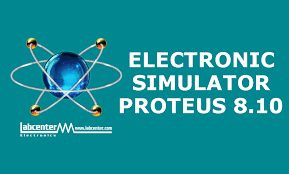
\includegraphics[scale= 1.5]{Chapter3/proteus}
%\caption{Simplified Block Diagram of Electronic Voting Machine(EVM) Using 8051 Microcontroller}
%\label{blockDiagram}
\end{center}
\end{figure}

\chapter{Simulation and Results}
\label{chap4}
In the previous chapter, we have discussed about our methodology for this project while giving details about block diagram, components selection of this project. In this chapter, we will provide source code, and simulation and results of the project.
\section{Simulation Results}
As discussed in the previous chapter in the section of software selection, we have used Proteus to simulate our project.
\section{Circuit Diagram}
Figure \ref{simulation1} shows circuit diagram of the project, which illustrates the main components involved
in Electronic Voting Machine(EVM) Using 8051 Micro-controller. Switches are used to make choices, resister, capacitor, and oscillator are being used to work the micro-controller properly on the circuits with the help of connecting wires.
\begin{figure}[H]  %h=positioning
\begin{center}
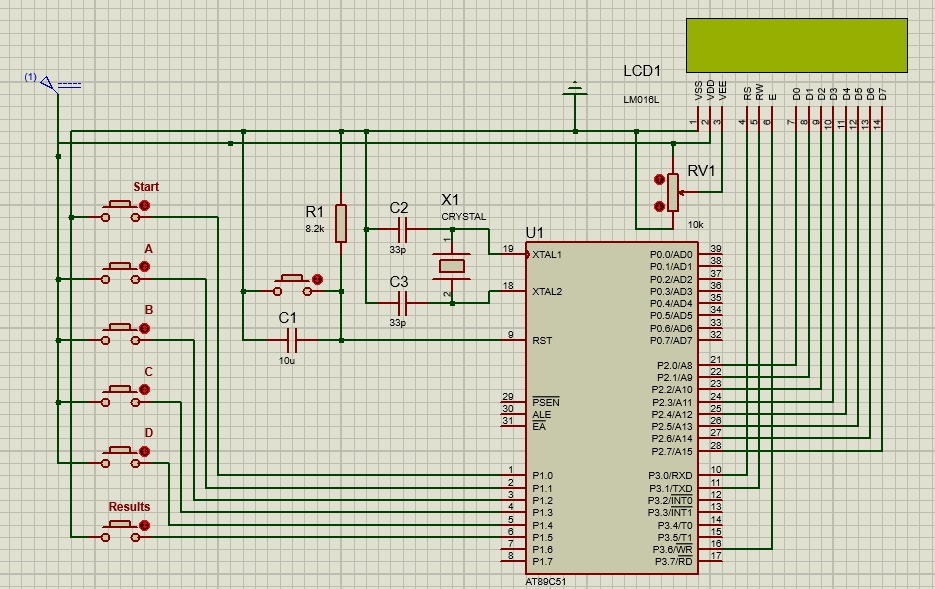
\includegraphics[scale=0.40]{Chapter4/simulation1}
\caption{Circuit Diagram of Electronic Voting Machine(EVM) Using 8051 Microcontroller}
\label{simulation1}
\end{center}
\end{figure}
\section{Source Code}
\begin{lstlisting}[frame=single]
#include<reg51.h>
#define msec 50
#define lcd_data_str_pin P2
sbit rs = P3^0;                  //Register select (RS) pin rs=0 command mode, rs=1 datamode
sbit rw = P3^1;                  //Read write(RW) pin rw=0 write mode, rw=1 read mode
sbit en = P3^6;                  //Enable(EN) pin



sbit ini_pin = P1^0;               // Start voting pin
sbit stop_pin = P1^5;            // Stop voting pin
sbit candidate_1=P1^1;                //Candidate1
sbit candidate_2=P1^2;              //Candidate2
sbit candidate_3=P1^3;                //Candidate3
sbit candidate_4=P1^4;             //Candidate4



int max = 0;
int carry = 0;
int arr[4];             //arry ofsize 4

int vote_amt[3],j;
unsigned int vote_1,vote_2,vote_3,vote_4;

void delay(int delay_time)                           // Time delay function
{

int j,k;
for(j=0;j<=delay_time;j++)
for(k=0;k<=1275;k++);
}

void lcd_cmd(unsigned char cmd_addr)                       //Function to send command to LCD
{
lcd_data_str_pin = cmd_addr;
en = 1;
rs = 0;
rw = 0;
delay(1);
en = 0;
return;
}

void lcd_data_str(char str[50])                               //Function to send string
{
int p;
for (p=0;str[p]!='\0';p++)
{
lcd_data_str_pin = str[p];
rw = 0;
rs = 1;
en = 1;

delay(1);
en = 0;
}
return;
}

void lcd_data_int(unsigned int vote)                        //Function to send 0-9 character values
{
char dig_ctrl_var;
int p;
for (j=2;j>=0;j--)
{
vote_amt[j]=vote%10;
vote=vote/10;
}

for (p=0;p<=2;p++)
{
dig_ctrl_var = vote_amt[p]+48;
lcd_data_str_pin = dig_ctrl_var;
rw = 0;
rs = 1;
en = 1;
delay(1);
en = 0;

}
return;
}

void vote_count()                                               // Function to count votes
{
while (candidate_1==0 && candidate_2==0 && candidate_3==0 && candidate_4==0);
if (candidate_1==1)
{
while (candidate_1 == 1);
{
vote_1 = vote_1 + 1;
}
}

if (candidate_2==1)
{
while (candidate_2 == 1);
{
vote_2 = vote_2 + 1;
}
}

if (candidate_3==1)
{
while (candidate_3 == 1);
{
vote_3 = vote_3 + 1;
}
}

if (candidate_4==1)
{
while (candidate_4 == 1);
{
vote_4 = vote_4 + 1;
}
}
}

void lcd_ini()
{
lcd_cmd(0x38);        //5x7 matrix 2 lines
delay(msec);
lcd_cmd(0x0E);                  //cursor on
delay(msec);
lcd_cmd(0x01);               //clear screen
delay(msec);
lcd_cmd(0x81);                //cursor position to 1st
delay(msec);
lcd_data_str("welcome here");
delay(100);
lcd_cmd(0x01);           //clear
delay(msec);
lcd_cmd(0x80);             //cursor position to 0 of line 1
delay(msec);
lcd_data_str( "you" );
delay(msec);
lcd_cmd(0x14);                     //space between
delay(msec);
lcd_data_str("can now");
delay(msec);
delay(msec);
lcd_cmd(0xC0);                 // second line
delay(msec);
lcd_data_str("cast your");
delay(msec);
lcd_cmd(0x14);                 // space
delay(msec);
lcd_data_str("vote");
delay(100);
lcd_cmd(0x01);                 //clear lcd
delay(msec);
lcd_cmd(0x80);                 //cursor position to 0 of line 1
delay(msec);
lcd_data_str("A");
delay(msec);
lcd_cmd(0x84);               // 4th col
delay(msec);
lcd_data_str("B");
delay(msec);
lcd_cmd(0x88);               // 8th col
delay(msec);
lcd_data_str("C");
delay(msec);
lcd_cmd(0x8C);                 // 12 col
delay(msec);
lcd_data_str("D");
delay(msec);
vote_count();
lcd_cmd(0x01);              //clear lcd
delay(msec);
lcd_cmd(0x83);             //ist line 3rd col
delay(msec);
lcd_data_str("thank");
delay(msec);
lcd_cmd(0x14);                 //space
delay(msec);
lcd_data_str("you");
delay(100);
}

void results()                // Function to show results
{
int i;
carry = 0;
lcd_cmd(0x01);                           //clear lcd
delay(msec);
lcd_cmd(0x80);                           //cursor position to 0 of line 1
delay(msec);
lcd_data_str("results");
delay(msec);
lcd_cmd(0x14);                        //space
delay(msec);
lcd_data_str("are");
delay(msec);
lcd_cmd(0x14);                         //space
delay(msec);
lcd_data_str("out");
delay(msec);
lcd_cmd(0x01);                         //clear lcd
delay(msec);
lcd_cmd(0x80);                         //cursor position to 0 of line 1
delay(msec);
lcd_data_str("A");
delay(msec);
lcd_cmd(0x84);                          //4th col
delay(msec);
lcd_data_str("B");
delay(msec);
lcd_cmd(0x88);                          // 8th col
delay(msec);
lcd_data_str("C");
delay(msec);
lcd_cmd(0x8C);                          // 12th col
delay(msec);
lcd_data_str("D");
delay(msec);
lcd_cmd(0xC0);                    //second line
delay(100);

lcd_data_int(vote_1);
delay(msec);
lcd_cmd(0xC4);                      //jump to 2nd line 4th row
delay(msec);
lcd_data_int(vote_2);
delay(msec);
lcd_cmd(0xC8);                      // 2nd line 8th row
delay(msec);
lcd_data_int(vote_3);
delay(msec);
lcd_cmd(0xCC);                   // 2nd line 12th row
delay(msec);
lcd_data_int(vote_4);
delay(300);

arr[0] = vote_1;                      //arry ofsize 4
arr[1] = vote_2;
arr[2] = vote_3;
arr[3] = vote_4;

for( i=0; i<4; i++)
{
if(arr[i]>=max)
max = arr[i];
}

if ( (vote_1 == max) && ( vote_2 != max) && (vote_3 != max)&& (vote_4 != max) )
{

carry = 1;
lcd_cmd(0x01);            //clear lcd
delay(msec);
lcd_cmd(0x80);              //cursor position to 0 of line 1
delay(msec);
lcd_data_str("congratulations");
delay(50);
lcd_cmd(0xC4);        //jump to 2nd line 4th col
delay(msec);
lcd_data_str("A");
delay(msec);
lcd_cmd(0x14);               //space
delay(msec);
lcd_data_str("wins");
delay(msec);
}

if ( (vote_2 == max) && ( vote_1 != max) && (vote_3 != max)&& (vote_4 != max) )
{
carry = 1;
lcd_cmd(0x01);     //clear lcd
delay(msec);
lcd_cmd(0x80);           //cursor position to 0 of line 1
delay(msec);
lcd_data_str("congratulations");
delay(50);
lcd_cmd(0xC4);                               //jump to 2nd line 4th col
delay(msec);
lcd_data_str("B");
delay(msec);
lcd_cmd(0x14);                 //space
delay(msec);
lcd_data_str("wins");
delay(msec);
}

if ( (vote_3 == max) && ( vote_2 != max) && (vote_1 != max)&& (vote_4 != max) )
{
carry = 1;
lcd_cmd(0x01);               //clear lcd
delay(msec);
lcd_cmd(0x80);                         //cursor position to 0 of line 1
delay(msec);
lcd_data_str("congratulations");
delay(50);
lcd_cmd(0xC4);                           ////jump to 2nd line 4th col
delay(msec);
lcd_data_str("C");
delay(msec);
lcd_cmd(0x14);                  //space
delay(msec);
lcd_data_str("wins");
delay(msec);
}

if ( (vote_4 == max) && ( vote_2 != max) && (vote_3 != max)&& (vote_1 != max) )
{
carry = 1;
lcd_cmd(0x01);     //clear lcd
delay(msec);
lcd_cmd(0x80);                          //cursor position to 0 of line 1
delay(msec);
lcd_data_str("congratulations");
delay(50);
lcd_cmd(0xC4);                      //jump to 2nd line 4th col
delay(msec);
lcd_data_str("D");
delay(msec);
lcd_cmd(0x14);                  //space
delay(msec);
lcd_data_str("wins");
delay(msec);
}

if (carry==0)

{
lcd_cmd(0x01);                 //clear lcd
delay(msec);
lcd_cmd(0x82);                //ist line 2nd col
delay(msec);
lcd_data_str("clash");
delay(50);
lcd_cmd(0x14);               //space
delay(msec);
lcd_data_str("between");
delay(50);
if(vote_1 == max)
{
lcd_cmd(0xC2);              //2nd line 2nd col
lcd_data_str("A");
delay(50);
}
if(vote_2 == max)
{
lcd_cmd(0xC5);                  //2nd line 5th col
lcd_data_str("B");
delay(50);
}
if(vote_3 == max)
{
lcd_cmd(0xC9);                      //2nd line 9th col
lcd_data_str("C");
delay(50);
}
if(vote_4 == max)
{
lcd_cmd(0xCD);                          //2nd line 12th col
lcd_data_str("D");
delay(50);
}
}
}

void main()
{
ini_pin = stop_pin = 1;
vote_1 = vote_2 = vote_3 = vote_4 = 0;
candidate_1 = candidate_2 = candidate_3 = candidate_4 = 0;
lcd_cmd(0x38);               //5x7 matrix 2 lines
delay(msec);
lcd_cmd(0x0E);               //cursor on
delay(msec);
lcd_cmd(0x01);                 //clear lcd
delay(msec);
lcd_cmd(0x80);              //cursor to fisrt pos
delay(msec);
lcd_data_str( "press b1" );
delay(msec);
lcd_cmd(0x14);               //sapce
delay(msec);
lcd_data_str("to");
delay(msec);
lcd_cmd(0xC0);                 // second line
delay(msec);
lcd_data_str("start");
delay(100);
while(1)
{
while(ini_pin != 0)
{
if (stop_pin == 0)
break;
}
if (stop_pin == 0)            //result pin
{
break;
}
lcd_ini();
}

while(1)
{
results();
}
}
\end{lstlisting}
\clearpage
\section{Results}
Following screen shot will show the step wise results which showed up as we run the project.
\begin{figure}[H]  %h=positioning
\begin{center}
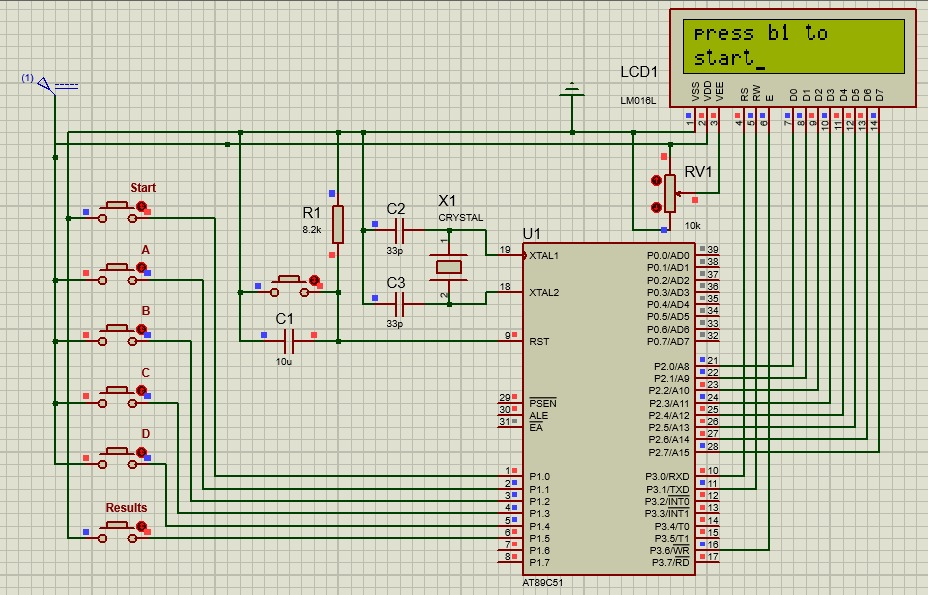
\includegraphics[scale=0.50]{Chapter4/simulation3}
%\caption{Circuit Diagram of Electronic Voting Machine(EVM) Using 8051 Microcontroller}
%\label{simulation1}
\end{center}
\end{figure}
\begin{figure}[H]  %h=positioning
\begin{center}
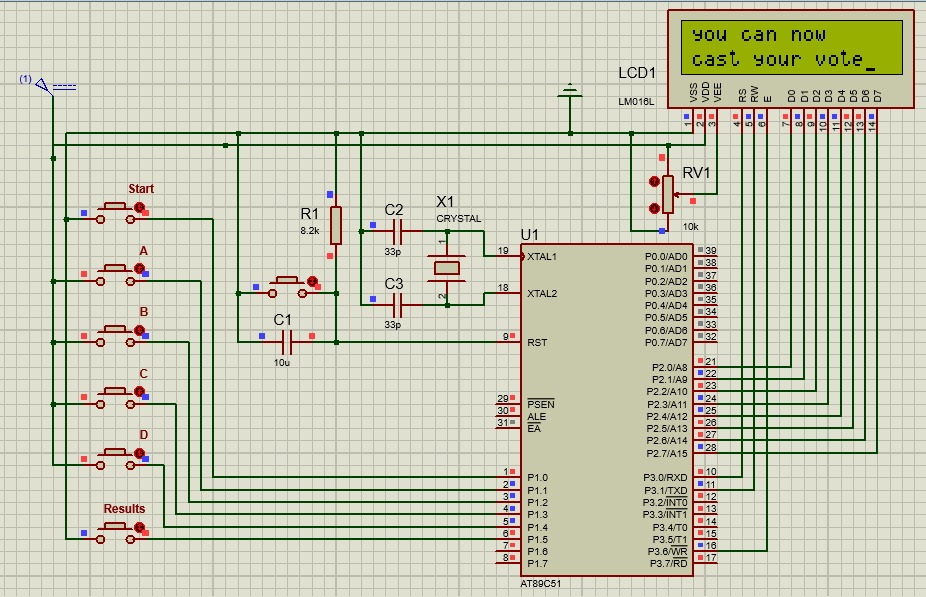
\includegraphics[scale=0.50]{Chapter4/simulation4}
%\caption{Circuit Diagram of Electronic Voting Machine(EVM) Using 8051 Microcontroller}
%\label{simulation1}
\end{center}
\end{figure}
\begin{figure}[H]  %h=positioning
\begin{center}
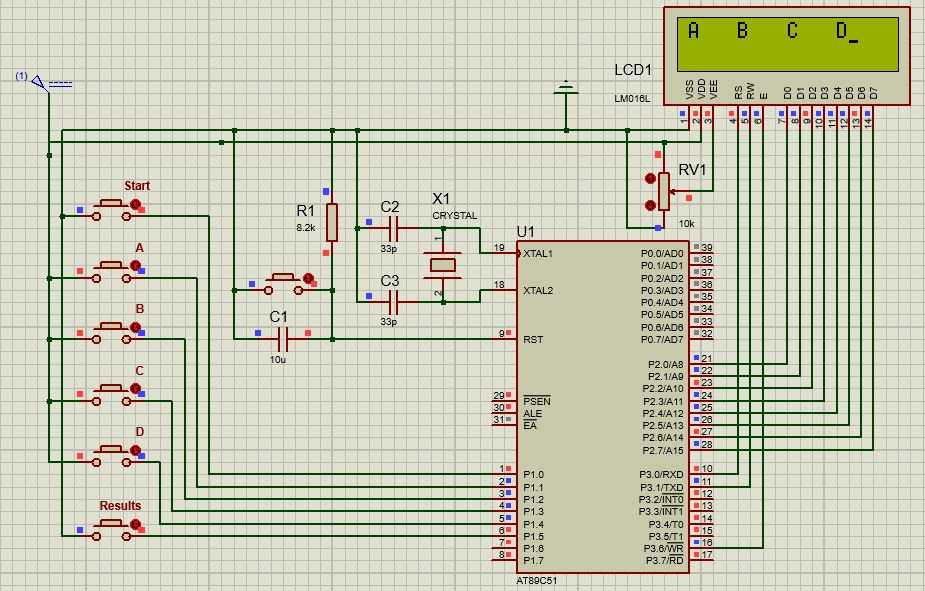
\includegraphics[scale=0.50]{Chapter4/simulation5}
%\caption{Circuit Diagram of Electronic Voting Machine(EVM) Using 8051 Microcontroller}
%\label{simulation1}
\end{center}
\end{figure}
\begin{figure}[H]  %h=positioning
\begin{center}
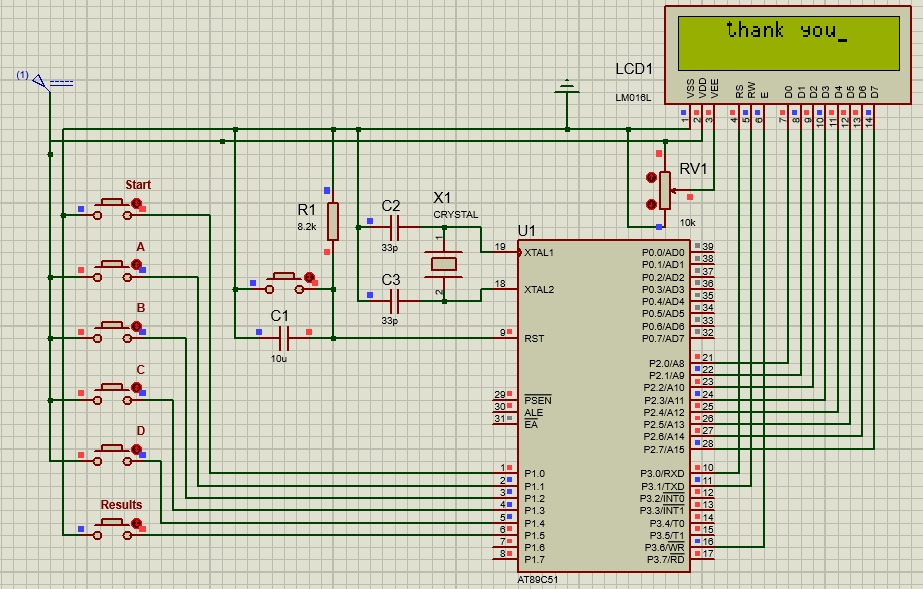
\includegraphics[scale=0.50]{Chapter4/simulation6}
%\caption{Circuit Diagram of Electronic Voting Machine(EVM) Using 8051 Microcontroller}
%\label{simulation1}
\end{center}
\end{figure}
\begin{figure}[H]  %h=positioning
\begin{center}
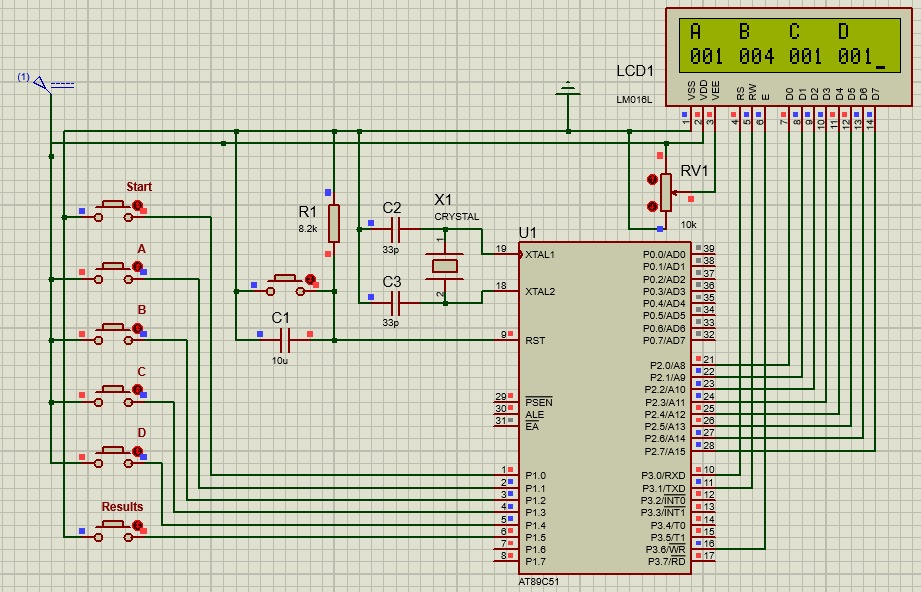
\includegraphics[scale=0.50]{Chapter4/simulation7}
%\caption{Circuit Diagram of Electronic Voting Machine(EVM) Using 8051 Microcontroller}
%\label{simulation1}
\end{center}
\end{figure}
\begin{figure}[H]  %h=positioning
\begin{center}
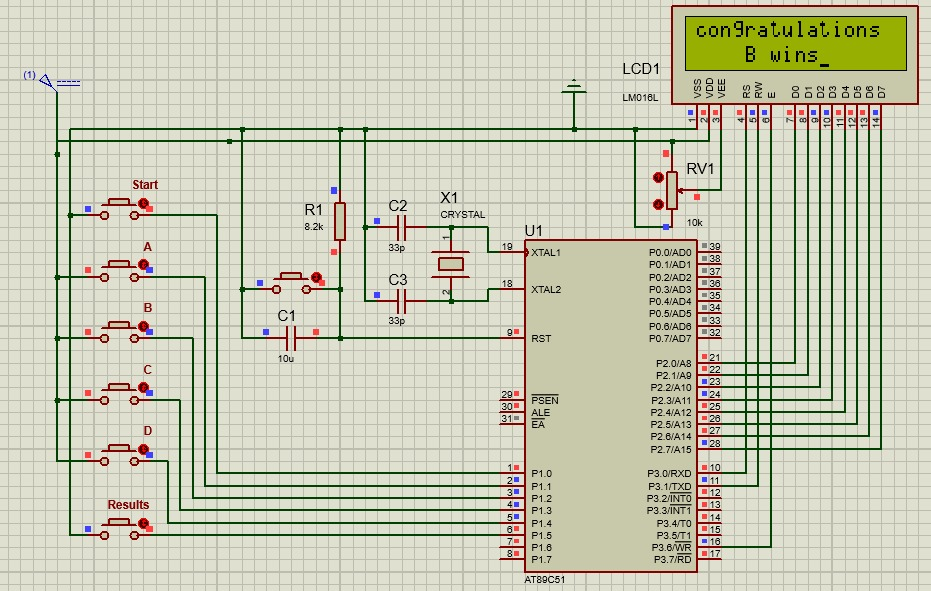
\includegraphics[scale=0.50]{Chapter4/simulation8}
%\caption{Circuit Diagram of Electronic Voting Machine(EVM) Using 8051 Microcontroller}
%\label{simulation1}
\end{center}
\end{figure}
\begin{figure}[H]  %h=positioning
\begin{center}
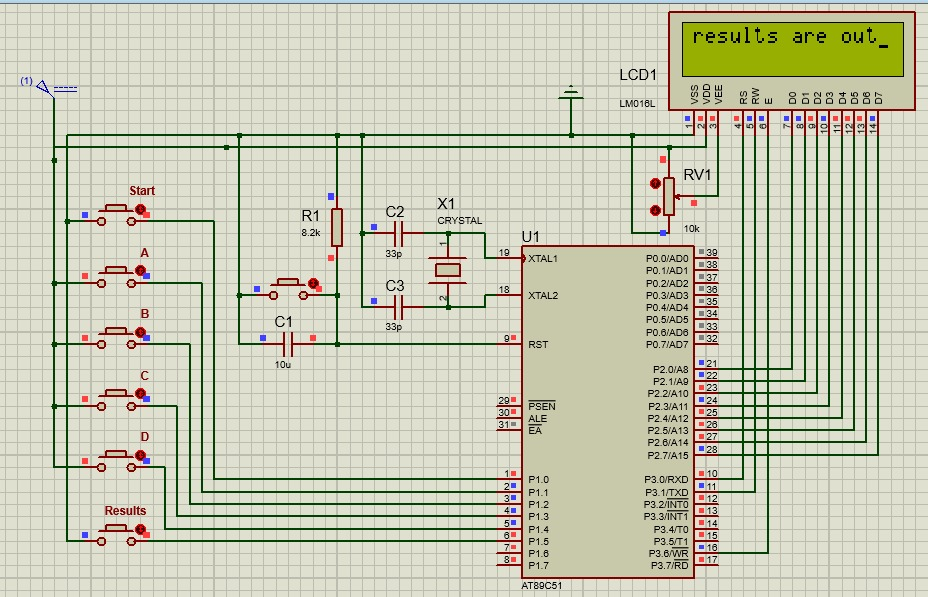
\includegraphics[scale=0.50]{Chapter4/simulation9}
%\caption{Circuit Diagram of Electronic Voting Machine(EVM) Using 8051 Microcontroller}
%\label{simulation1}
\end{center}
\end{figure}
\section{Hardware Implementation}
\begin{figure}[H]  %h=positioning
\begin{center}
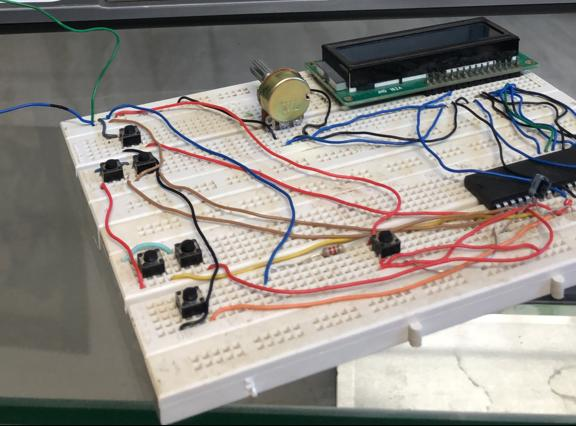
\includegraphics[scale=0.65]{Chapter4/hardware1}
\caption{Hardware Implementation of Electronic Voting Machine(EVM) Using 8051 Microcontroller}
\label{hardware1}
\end{center}
\end{figure}

\chapter{Conclusion and Future Work}
\label{chap5}
In the previous chapter, we have shown all the simulation and results of our proposed project from introduction, literature review, proposed methodology, result and simulations. In this chapter, we will conclude our project and will give some future works recommendations.
\section{Conclusion}
This work describes the working of Electronic Voting Machine. We have:
\begin{enumerate}
\item Lesser chance of rigging in the elections
%
\item From Ballot paper now elections will be automated
%
\item The elections will be now time efficient and cost efficient
%
\end{enumerate}


\section{Future Work}
Electronic Voting Machine can be done in many other ways and the current method/project can be improve in many ways. Following are the some of the things we can try to improve this system:
\begin{enumerate}
\item Different microcontroller can be used to improve it.
%
\item Can work on this to improve the system accuracy.
%
%
\item Can use fingerprint, or face recognition technique to better person identification.
\end{enumerate}


%\include{Chapter6/Chapter6}
%\include{Chapter8/Chapter8}
%\include{Chapter7/Chapter7}

\bibliographystyle{ieeetr}
\bibliography{Ref}
\end{document}
